\فصل{پیاده‌سازی و ارزیابی}

در این پژوهش تولید سلسله فعالیت جعلی به نحوی که از دید سکو قابل تمایز با سلسله فعالیت واقعی نباشد؛ نیاز به پیاده‌سازی دقیق مدل‌سازی مطرح شده در بخش \ref{chapter:c44} و ارزیابی کامل بر اساس مدل تهدید گفته شده در بخش \ref{chapter:c42} است. در این فصل به توصیف کلی پیاده‌سازی نرم‌افزار و ارزیابی کامل آن با نمونه داده‌های متنوع بر اساس مدل تهدید سکوی بدخواه خواهیم پرداخت.

\section{پیاده‌سازی}

در این بخش به بررسی پیاده‌سازی راهکار پیشنهادی این پژوهش طبق الگوریتم گفته شده در بخش \ref{chapter:c443} می‌پردازیم.

\subsection{معماری و ساختار پیاده‌سازی}

راهکار پیشنهادی این پژوهش به صورت یک پروژه \lr{Web API} است که به زبان \پاورق{‌سی‌شارپ}{C\#} توسعه یافته است. پروژه های \lr{Web API} به عنوان واسط‌هایی عمل می‌کنند که امکان ارتباط بین برنامه‌های مختلف را از طریق پروتکل \lr{HTTP} فراهم می‌سازند و به گونه‌ای طراحی شده‌اند که سرویس‌های مختلفی را از طریق اینترنت یا شبکه‌های داخلی در دسترس قرار دهند \cite{xp1}. در این پروژه، \پاورق{‌\lr{API}}{Application Programming Interface}ها به‌طور کامل مستندسازی شده‌اند و از طریق ابزار \lr{Swagger} قابل دسترسی و بررسی هستند. \lr{Swagger} به کاربران و توسعه‌دهندگان این امکان را می‌دهد که به‌راحتی با عملکرد \lr{API}ها آشنا شوند، درخواست‌های مختلف را آزمایش کنند و مستندات مربوط به هر سرویس را مشاهده نمایند \cite{xp2}.

راهکار پیشنهادی این پژوهش با استفاده از \پاورق{‌معماری سه لایه}{Three Layered Architecture} طراحی شده است که شامل لایه‌های \lr{API}، \پاورق{‌دامنه}{Domain} و \پاورق{‌زیرساخت}{Infrastructure} می‌باشد. لایه \lr{API} به عنوان رابط کاربری عمل می‌کند و درخواست‌ها را از کاربران دریافت کرده و به لایه دامنه ارسال می‌کند. لایه دامنه مسئولیت مدیریت منطق کسب‌وکار و پردازش داده‌ها را بر عهده دارد. لایه زیرساخت نیز ارتباط با پایگاه داده و منابع خارجی را فراهم می‌سازد \cite{xp3}.

برای مدیریت داده‌ها در این راهکار پیشنهادی این پژوهش از \lr{SQL Server} استفاده شده است. این پایگاه داده به عنوان \پاورق{‌سیستم مدیریت پایگاه داده}{Database Management System (DBMS)} عمل می‌کند و داده‌های پروژه را به صورت ساختاریافته ذخیره و مدیریت می‌نماید، که این امر باعث افزایش کارایی و سرعت دسترسی به داده‌ها می‌شود \cite{xp4}.

\subsection{کد برنامه}

عملکرد اصلی راهکار پیشنهادی این پژوهش در کلاس \lr{CoreService} انجام شده است که بخش‌های اصلی آن را به صورت دقیق تعریف می‌کنیم.

\begin{itemize}
\item \textbf{\lr{GenerateFakeActivities}}: در این تابع با توجه به شرایط کنونی خانه هوشمند، به صورت عقبگرد حرکت کرده تا به نقطه شروع تولید سلسله فعالیت جعلی برسیم (ممکن است شرایط کنونی ورود به خانه باشد و نیازی به جرکت عقبگرد نداشته باشیم).
\item \textbf{\lr{CheckConditions}}: در این تابع شرایط انجام فعالیتی که می‌خوایم به سلسله فعالیت جعلی اضافه شود را بررسی می‌کنیم تا با توجه به حالت خانه هوشمند، فعالیت قابل انجام باشد.
\item \textbf{\lr{GenerateRecursively}}: در این تابع تولید سلسله فعالیت جعلی انجام می‌شود و در هر مرحله با توجه به فعالیت‌های بعدی ممکن، یک مرحله جلو می‌رویم تا به نقطه‌ توقف برسیم.
\item \textbf{\lr{SetResults}}: پس از تولید هر فعالیت جعلی، تغییر حالت خانه هوشمند که نتیجه آن فعالیت است را اعمال می‌کنیم تا حالت خانه هوشمند از دید سکو، حالتی منطقی و درست باشد.
\item \textbf{\lr{FindNextActivity}}: در این تابع از بین فعالیت ممکن قابل انجام پس از فعالیت جعلی تولید شده، یکی را به صورت تصادفی (با احتمال انجام آن بر اساس قوانین انجمنی) انتخاب می‌کنیم.
\item \textbf{\lr{GenerateFinalResult}}: در این تابع که پس از اتمام تابع \lr{GenerateRecursively} اجرا می‌شود، هر فعالیت به داده‌های ارسالی حسگرها نگاشت می‌شود تا به سکو ارسال شوند.
\end{itemize}

\section{ارزیابی}

برای ارزیابی این پژوهش میزان گمراه‌سازی سکو با تولید رخدادهای جعلی بر اساس مجموعه داده‌ای از فعالیت‌های کاربر توسط ابزار پیاده‌سازی شده اندازه‌گیری شده است. بدین منظور ابتدا هستی‌شناسی متناسب با مجموعه داده تعریف شده و پس از تولید سلسله فعالیت جعلی، ترکیب آن با سلسله فعالیت واقعی به دسته‌بند داده شده و میزان کاهش دقت آن به عنوان معیار ارزیابی در نظر گرفته شده است. این معیار نشان‌دهنده‌ قدرت راهکار پیشنهادی در گمراه‌سازی سکو است.

\subsection{مجموعه دادگان}

مجموعه داده مورد استفاده در این پژوهش مجموعه داده \lr{Orange4Home} \cite{xyz6} است که شامل تقریباً ۱۸۰ ساعت فعالیت‌های روزمره یک فرد است که به مدت ۴ هفته متوالی در روزهای کاری انجام شده است. این مجموعه داده شامل داده‌های ۲۳۶ حسگر ناهمگن است که به‌طور یکپارچه در سراسر یک آپارتمان پخش شده‌اند و ۲۰ دسته فعالیت که توسط فرد به‌طور دقیق در محل برچسب‌گذاری شده‌اند، و در مجموع ۴۹۳ نمونه از فعالیت‌ها را شامل می‌شود. این ویژگی‌ها، \lr{Orange4Home} را به یک مجموعه داده مناسب برای ارزیابی الگوریتم‌های شناسایی فعالیت، ارزیابی الگوریتم‌های پیش‌بینی فعالیت و سایر مسائل پژوهشی مرتبط با الگوریتم‌ها و خانه‌های هوشمند تبدیل می‌کند.

خانه هوشمند استفاده شده در مجموعه داده \lr{Orange4Home} شامل بخش‌های ورودی، آشپزخانه، دستشویی، پذیرایی و راه پله در طبقه همکف و راه پله، راهرو، دفتر کار، حمام و اتاق خواب در طبقه اول است که این نقشه در اشکال \ref{fig:fO4H1} و  \ref{fig:fO4H2} قابل مشاهده است.

\begin{figure}[H]
\centerline{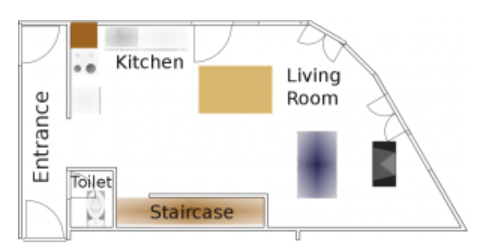
\includegraphics[width=0.8\textwidth]{figs/fO4H1.png}}
\caption{نقشه خانه مجموعه داده \lr{Orange4Home}، طبقه همکف}
\label{fig:fO4H1}
\end{figure}

\begin{figure}[H]
\centerline{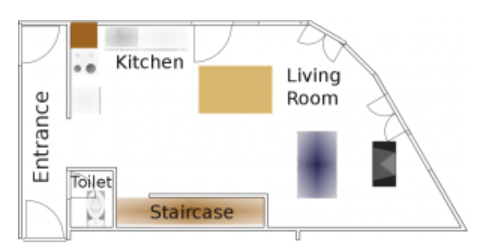
\includegraphics[width=0.8\textwidth]{figs/fO4H1.png}}
\caption{نقشه خانه مجموعه داده \lr{Orange4Home}، طبقه اول}
\label{fig:fO4H2}
\end{figure}

در هر بخش از این خانه هوشمند، حسگرهایی با انواع \پاورق{‌دودویی}{Binary}، \پاورق{‌عدد صحیح}{Integer}، \پاورق{‌عددی}{Real number} و \پاورق{‌دسته‌ای}{Categorical} وجود دارد که تعداد این حسگرها به تفکیک بخش‌های مختلف خانه هوشمند، در شکل \ref{tab:tO4H1} قابل مشاهده است. تعدادی از حسگرها در مجموعه داده \lr{Orange4Home} سراسری و برای کل خانه است که این مقادیر رابطه مستقیم با فعالیت فعلی کاربر و داده حسگرهای مربوط به فعالیت‌ها ندارند، در نتیجه در مجموعه داده و تولید سلسله فعالیت جعلی از این داده‌ها صرف نظر شده است و به جای 236 حسگر، در این پژوهش از 196 حسگر (با حذف حسگرهای سراسری) استفاده شده است.

\begin{table} [htp]
 \centering
 \caption{حسگرهای هر بخش خانه هوشمند}
 \label{tab:tO4H1}
 \begin{adjustbox}{width=0.8\textwidth}
\begin{tabular}{|l|c|c|c|c|c|}
\hline
\textbf{محل} & \textbf{دودویی} & \textbf{عدد صحیح} & \textbf{عددی} & \textbf{دسته‌ای} & \textbf{مجموع} \\ \hline
ورودی       & 3               & 1                & 2                    & 3                    & 9             \\ \hline
آشپزخانه        & 13              & 21               & 18                   & 0                    & 52            \\ \hline
پذیرایی    & 16              & 6                & 8                    & 7                    & 37            \\ \hline
دستشویی         & 3               & 1                & 1                    & 0                    & 5             \\ \hline
راه پله      & 3               & 0                & 0                    & 0                    & 3             \\ \hline
راهرو        & 9               & 0                & 1                    & 0                    & 10            \\ \hline
حمام       & 9               & 6                & 8                    & 3                    & 26            \\ \hline
دفتر کار         & 9               & 3                & 3                    & 5                    & 20            \\ \hline
اتاق خواب        & 17              & 4                & 6                    & 7                    & 34            \\ \hline
سراسری         & 1               & 13               & 20                   & 6                    & 40            \\ \hline
\textbf{مجموع} & \textbf{83}     & \textbf{55}      & \textbf{67}          & \textbf{31}          & \textbf{236}  \\ \hline
\end{tabular}
\end{adjustbox}
\end{table}

در این مجموعه داده فعالیت‌های برچسب‌گذاری شده شامل داده‌های حسگرها می‌باشند و تمامی اطلاعات ارسالی از حسگرها بین شروع و پایان برچسب یک فعالیت است. هر فعالیت‌های برچسب‌گذاری شده متعلق به یک بخش خانه است که در ادامه لیستی از این فعالیت‌ها را داریم:

\begin{itemize}
\item \textbf{ورودی}: ورود، خروج
\item \textbf{آشپزخانه}: آماده‌سازی، آشپزی، شستن ظروف
\item \textbf{پذیرایی}: خوردن، تلویزیون دیدن، کار با رایانه
\item \textbf{دستشویی}: استفاده از دستشویی
\item \textbf{راه پله}: بالا رفتن، پایین آمدن
\item \textbf{حمام}: استفاده از روشویی، استفاده از دستشویی، حمام کردن
\item \textbf{دفتر کار}: کار با رایانه، تلویزیون دیدن
\item \textbf{اتاق خواب}: لباس عوض کردن، کتاب خواندن، خوابیدن
\item \textbf{تمامی بخش‌ها}: تمیز کاری
\end{itemize}

همانطور که گفته شد، داده‌های حسگرها بین شروع و پایان یک فعالیت برچسب‌گذاری شده ارسال می‌شوند. در مجموعه داده \lr{Orange4Home}، یک فایل \lr{csv} قرار دارد که داده حسگرها با را در خود دارد. این داده‌ها شامل زمان دقیق ارسال داده توسط حسگر، نام حسگر و مقدار ارسال شده توسط آن حسگر است که نمونه داده‌ موجود در مجموعه داده در شکل \ref{fig:fO4H3} قابل مشاهده است. در این شکل شروع فعالیت ورود به خانه است که در همان دقیقه ورود و باز کردن درب، داده‌های مربوط به صدای محیط، روشن شدن چراغ و ... به صورت خودکار به سکو ارسال می‌گردد.

\begin{figure}[H]
\centerline{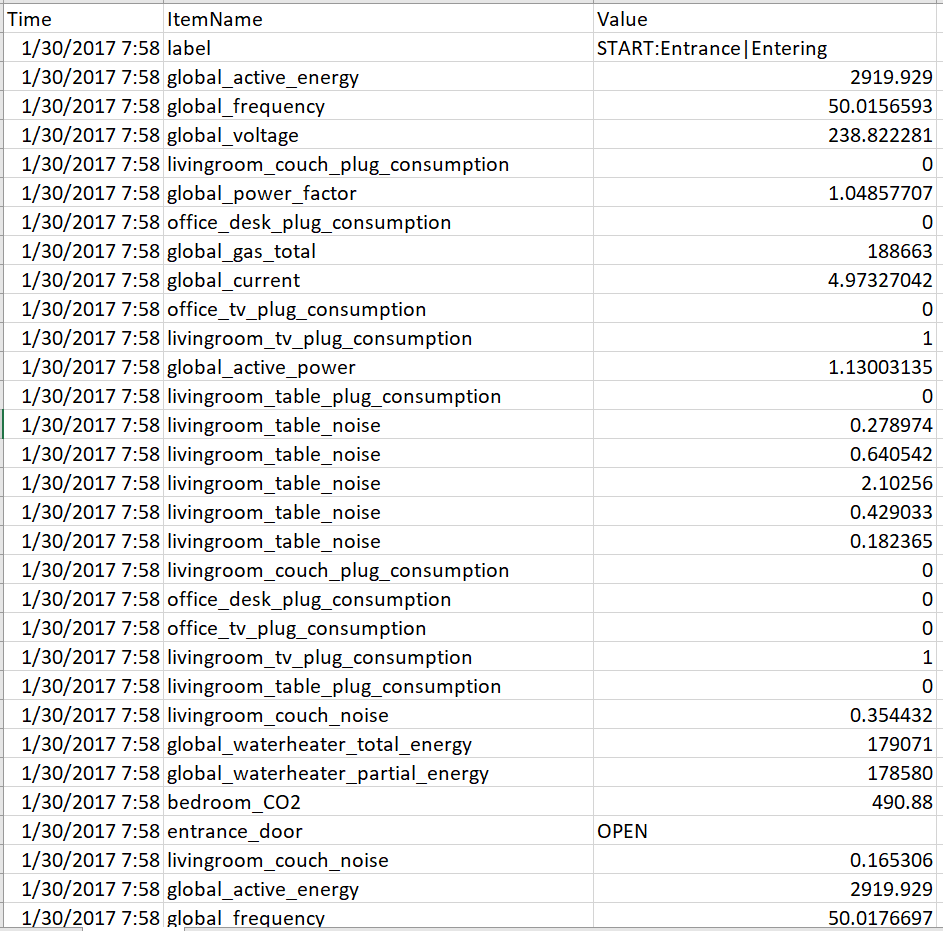
\includegraphics[width=0.8\textwidth]{figs/fO4H3.png}}
\caption{نمونه داده ارسالی از حسگرها}
\label{fig:fO4H3}
\end{figure}

\subsection{هستی‌شناسی}‌

برای استخراج هستی‌شناسی از مجموعه داده \lr{Orange4Home}، ابتدا مجاورت بخش‌های مختلف خانه بر اساس نقشه تعریف شده است. سپس نسخه‌ای فیلتر شده از مجموعه داده که فقط دارای فعالیت‌های برچسب‌گذاری شده است را تهیه کردیم که بخشی از آن در شکل \ref{fig:fO4H4} قابل مشاهده است. از این مجموعه داده برای محاسبه احتمال رخداد یک فعالیت پس از دیگری استفاده شده است تا بتوانیم سلسله فعالیت جعلی غیر قابل تمایز با استفاده از قوانین انجمنی تولید کنیم (جزئیات استفاده از احتمالات در قوانین انجمنی، در بخش \ref{chapter:c442} آورده شده است). 

\begin{figure}[H]
\centerline{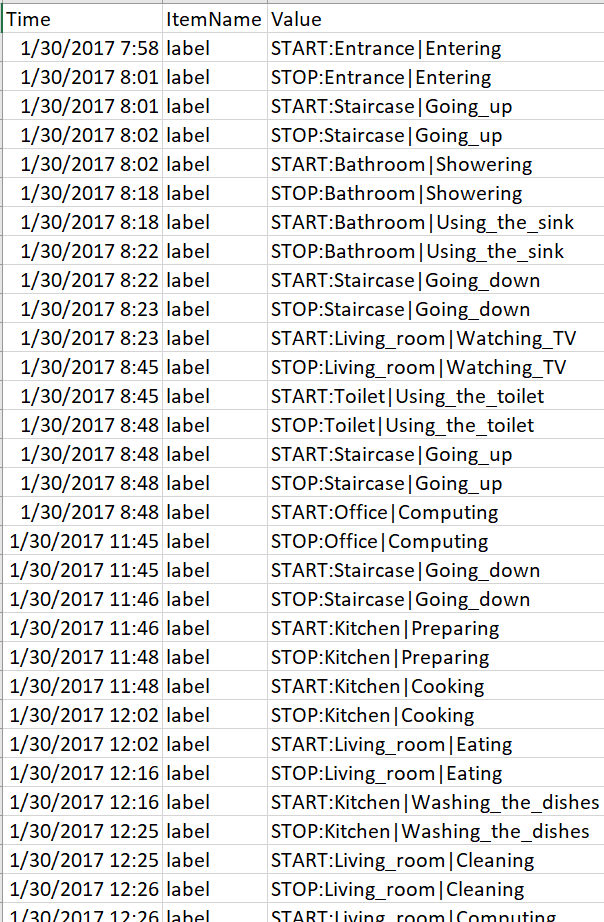
\includegraphics[width=0.8\textwidth]{figs/fO4H4.png}}
\caption{بخشی از مجموعه داده فیلتر شده که فقط فعالیت‌ها در آن هستند.}
\label{fig:fO4H4}
\end{figure}

سپس، داده حسگرها مربوط به هر فعالیت برچسب‌گذاری شده را استخراج میکنیم و پس از تولید سلسله فعالیت جعلی بر اساس هستی‌شناسی و  قوانین انجمنی فعالیت‌ها، به جای هر فعالیت یکی از سلسله داده حسگرهای موجود در مجموعه داده برای آن فعالیت را به صورت تصادفی انتخاب میکنیم و به سکو ارسال می‌کنیم. سلسله داده‌های ارسالی حسگرها به ازای هر فعالیت در هستی ‌شناسی آن فعالیت و ارتباط با حسگرها قرار داده شده است.

\subsection{دسته‌بند}‌

همان‌طور که بیان شد، برای ارزیابی کیفیت سلسله فعالیت‌ جعلی تولید شده توسط ابزار پیشنهادی، میزان افت دقت تشخیص فعالیت توسط یک دسته‌بند اندازه‌گیری می‌شود. برای این منظور از دسته‌بند استفاده شده در کار پژوهشی اقوامی و همکاران \cite{x3341} به عنوان معیار ارزیابی استفاده شده است که با دقت ۹۸ درصد فعالیت متناظر با رخدادهای مجموعه‌داده \lr{Orange4Home} را تشخیص می‌دهد. این دسته‌بند یک شبکه عصبی پیچشی است که معماری آن در شکل \ref{fig:fO4H5} آورده شده است. ورودی این دسته‌بند یک بردار شامل ۱۹۶ مقدار است که هر کدام نشانگر یک حسگر در خانه است و مقدار آن بیانگر آخرین رخداد گزارش شده از آن حسگر است. این مقادیر با پیش‌پردازش مجموعه داده محاسبه شده است و برای پر کردن مقادیر ناموجود در هر لحظه، از مقدار قبل از آن و یا در صورت عدم وجود، از مقدار بعد از آن استفاده شده است. بدین ترتیب دسته‌بند با داشتن یک وضعیت از تمام حسگرها، فعالیت کاربر در آن زمان را تشخیص می‌دهد.


\begin{figure}[H]
\centerline{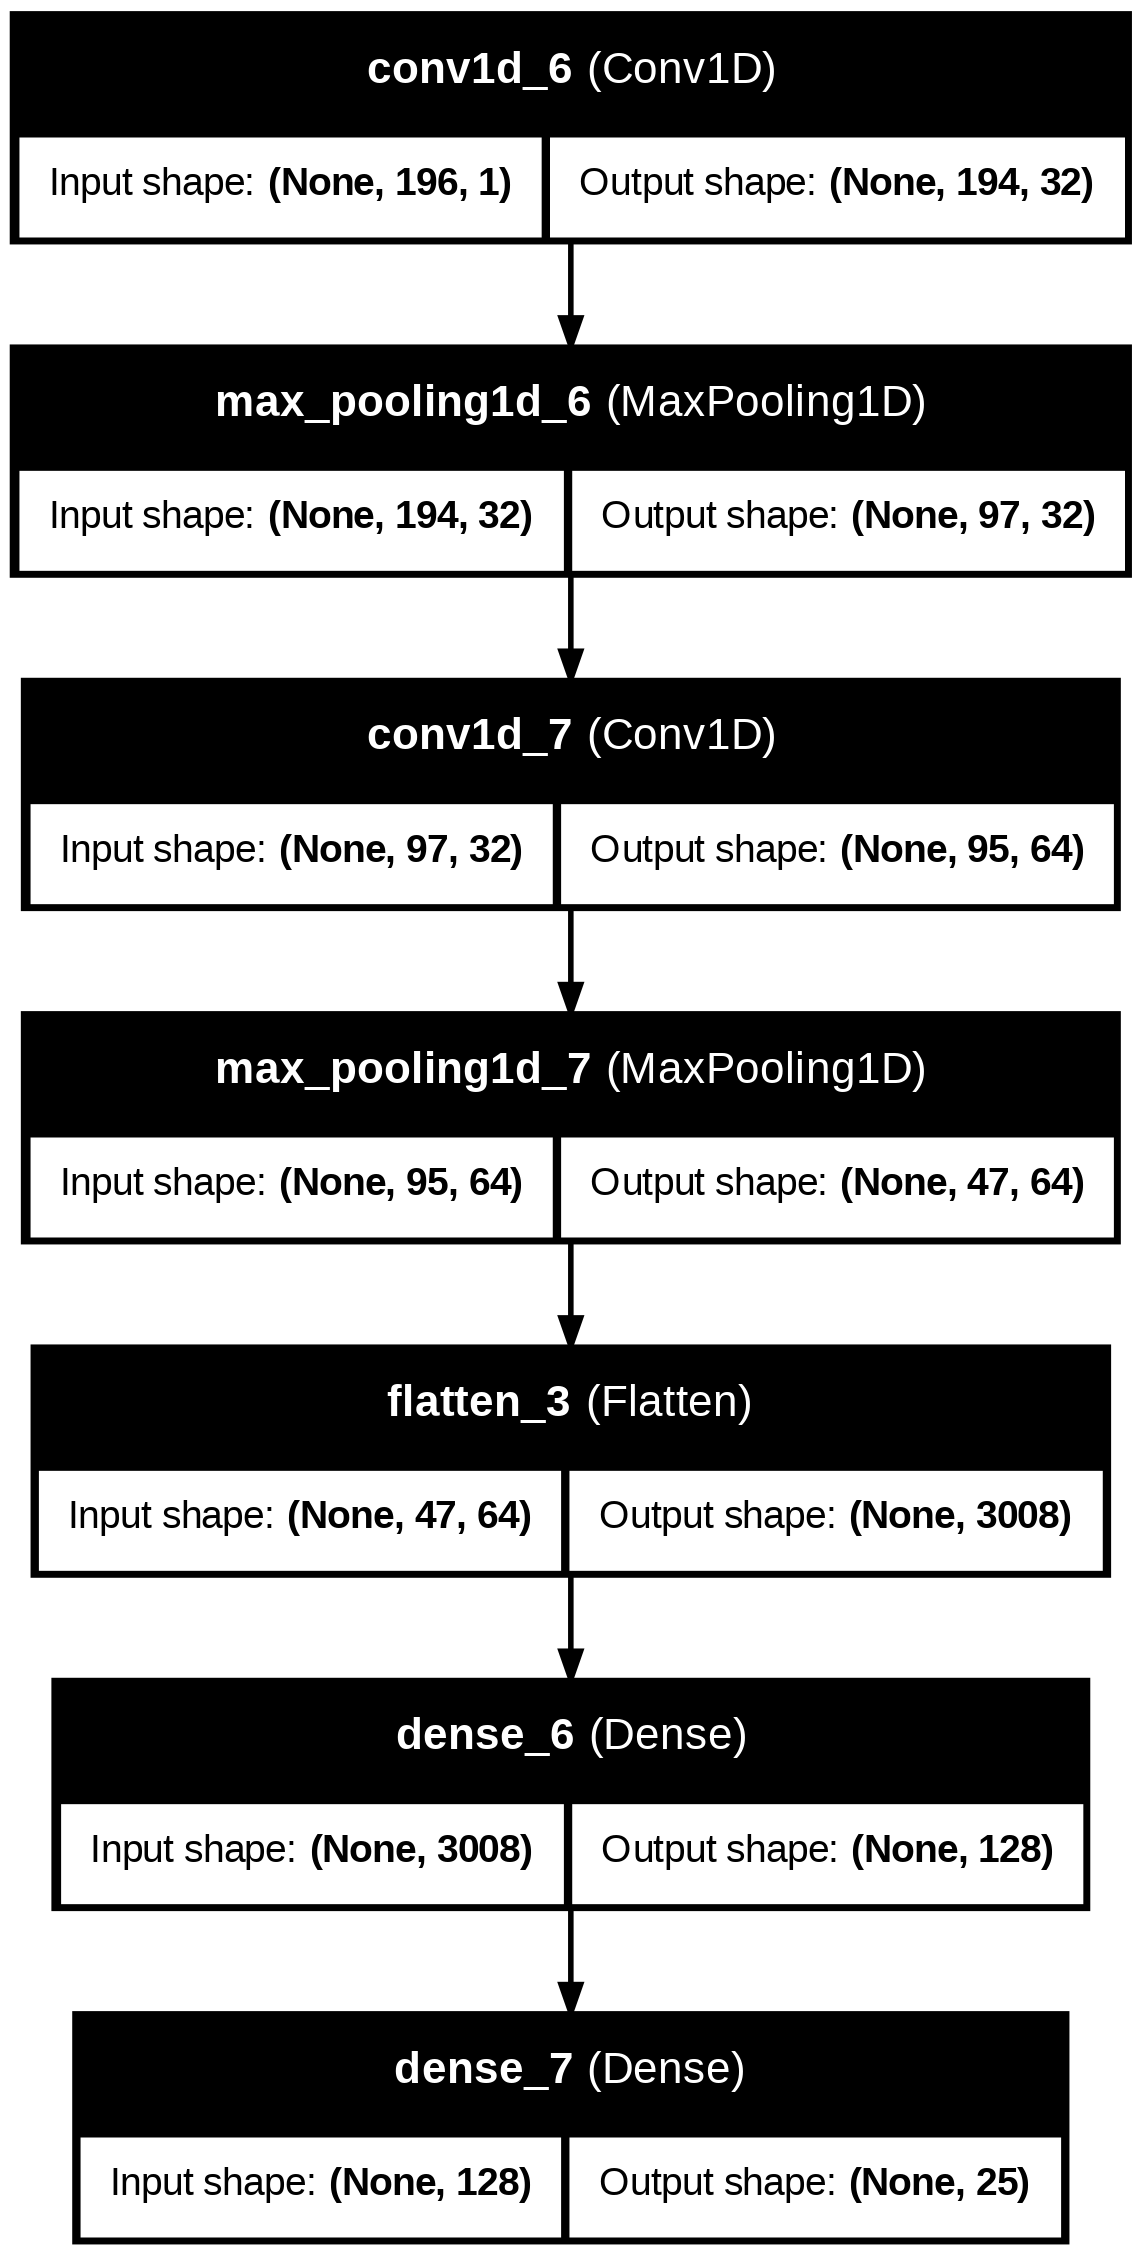
\includegraphics[width=0.5\textwidth]{figs/fO4H5.png}}
\caption{معماری دسته‌بند استفاده شده}
\label{fig:fO4H5}
\end{figure}

\subsection{نتایج}‌

ناقص. شکلی با کلیت \ref{fig:fnatijeh} خواهد داشت.

\begin{figure}[H]
\centerline{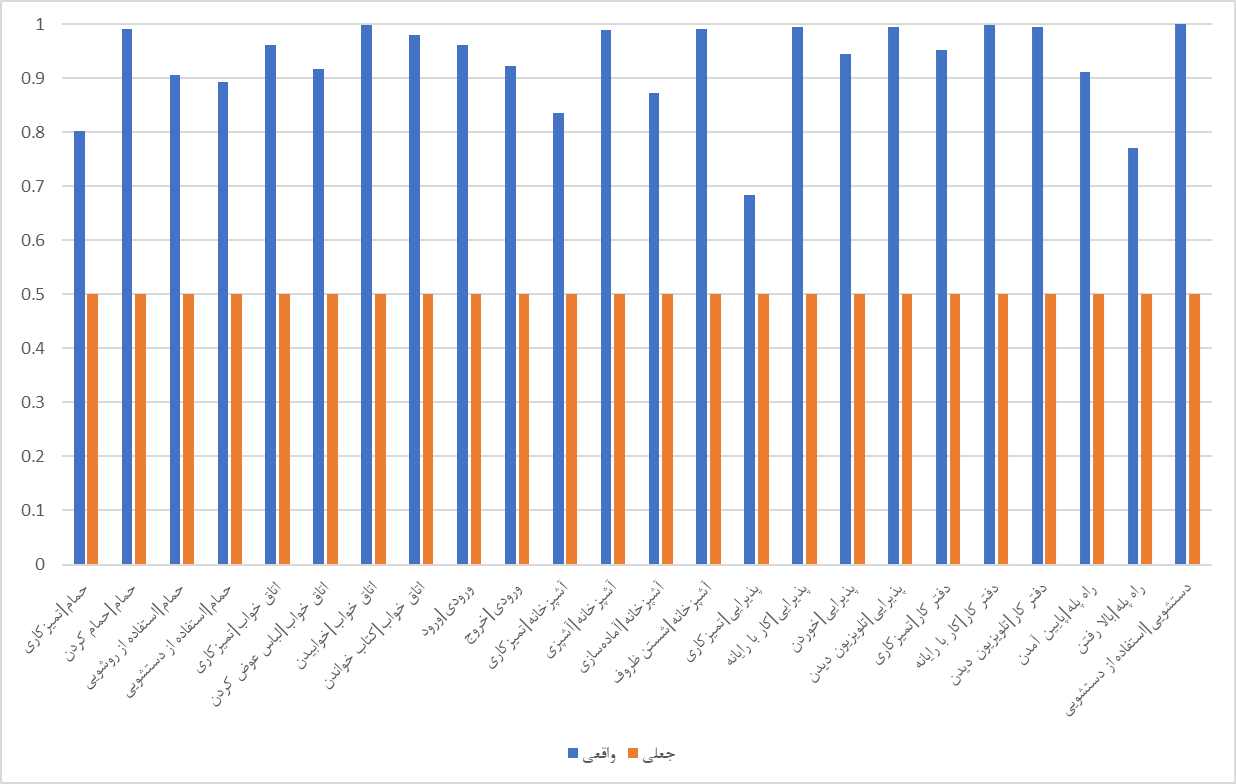
\includegraphics[width=0.5\textwidth]{figs/fnatijeh.png}}
\caption{نتیجه}
\label{fig:fnatijeh}
\end{figure}


